\documentclass[journal,12pt,onecolumn]{IEEEtran}
\usepackage{cite}
\usepackage{graphicx}
\usepackage{amsmath,amssymb,amsfonts,amsthm}
\usepackage{algorithmic}
\usepackage{graphicx}
\usepackage{textcomp}
\usepackage{xcolor}
\usepackage{txfonts}
\usepackage{listings}
\usepackage{enumitem}
\usepackage{mathtools}
\usepackage{gensymb}
\usepackage{comment}
\usepackage[breaklinks=true]{hyperref}
\usepackage{tkz-euclide} 
\usepackage{listings}
\usepackage{gvv}                                        
%\def\inputGnumericTable{}                                 
\usepackage[latin1]{inputenc} 
\usetikzlibrary{arrows.meta, positioning}
\usepackage{xparse}
\usepackage{color}                                            
\usepackage{array}                                            
\usepackage{longtable}                                       
\usepackage{calc}                                             
\usepackage{multirow}
\usepackage{multicol}
\usepackage{hhline}                                           
\usepackage{ifthen}                                           
\usepackage{lscape}
\usepackage{tabularx}
\usepackage{array}
\usepackage{float}
\newtheorem{theorem}{Theorem}[section]
\newtheorem{problem}{Problem}
\newtheorem{proposition}{Proposition}[section]
\newtheorem{lemma}{Lemma}[section]
\newtheorem{corollary}[theorem]{Corollary}
\newtheorem{example}{Example}[section]
\newtheorem{definition}[problem]{Definition}
\newcommand{\BEQA}{\begin{eqnarray}}
\newcommand{\EEQA}{\end{eqnarray}}
\usepackage{float}
\theoremstyle{remark}
\usepackage{circuitikz}
\usepackage{tikz} 
\graphicspath{{figs/}}

\title{GATE 2021 STATISTICS}
\author{EE25BTECH11022 - SANKEERTHAN }
\date{}


\begin{document}
\maketitle
\textbf{\underline{General Aptitude}}

\begin{enumerate}
\item 
The current population of a city is 11,02,500. If it has been increasing at the rate of $5\%$ per annum, what was its population 2 years ago?

\begin{enumerate}
\item 9,92,500
\item 9,95,006
\item 10,00,000
\item 12,51,506
\end{enumerate}

\hfill (GATE ST 2021)\\

\item If $p$ and $q$ are positive integers and
$
\frac{p}{q} + \frac{q}{p} = 3,
$
then
$
\frac{p^{2}}{q^{2}} + \frac{q^{2}}{p^{2}} = \ ?
$
\begin{enumerate}
\item 3
\item 7
\item 9
\item 11
\end{enumerate}

\hfill (GATE ST 2021) 


\item 

\begin{figure}[h]
    \centering
    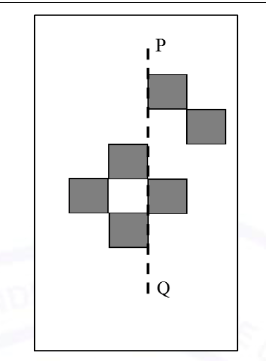
\includegraphics[width=0.2\linewidth]{figs/3.png}
    \caption{}
    \label{fig:1}
\end{figure}

The least number of squares that must be added so that the line P-Q becomes the line of symmetry is:

\begin{enumerate}
\item 4
\item 3
\item 6
\item 7
\end{enumerate}

\hfill (GATE ST 2021) \\



\item
Nostalgia is to anticipation as \_\_\_\_\_ is to \_\_\_\_\_.  
Which one of the following options maintains a similar logical relation?

\begin{enumerate}
\item Present, past
\item Future, past
\item Past, future
\item Future, present
\end{enumerate}
\hfill (GATE ST 2021)

 

\item
Consider the following sentences:
\begin{enumerate}
\item[(i)] I woke up from sleep.
\item[(ii)] I woked up from sleep.
\item[(iii)] I was woken up from sleep.
\item[(iv)] I was wokened up from sleep.
\end{enumerate}
Which of these sentences are grammatically correct?
\begin{enumerate}
\item (i) and (ii)
\item (i) and (iii)
\item (ii) and (iii)
\item (i) and (iv)
\end{enumerate}
\hfill (GATE ST 2021)\\



\item
Statements:  
1. All purple are green. \\ 
2. All black are green.  

Conclusions: 
I. Some black are purple.  \\
II. No black is purple.

Which option is logically correct?
\begin{enumerate}
\item Only I  
\item Only II  
\item Either I or II  
\item Both I and II
\end{enumerate}

\hfill (GATE ST 2021)\\
\item
Computers are ubiquitous... (passage given).  
Which of the following can be deduced?  
(i) Nowadays, computers are present in almost all places.  
(ii) Computers cannot be used for solving problems in engineering.  
(iii) Humans have both positive and negative effects from using computers.  
(iv) Artificial intelligence can be done without data.

\begin{enumerate}
\item (ii) and (iii)
\item (ii) and (iv)
\item (i), (iii) and (iv)
\item (i) and (iii)
\end{enumerate}

\hfill (GATE ST 2021)\\

\item
A square sheet of side 1 unit is cut along the diagonal.  
One triangle is revolved about its short edge to form a cone.  
Volume of the cone is:

\begin{enumerate}
\item $\frac{\pi}{3}$
\item $\frac{2\pi}{3}$
\item $\frac{3\pi}{2}$
\item $3\pi$
\end{enumerate}
\hfill (GATE ST 2021)\\

\newpage
\item
\begin{figure}
    \centering
    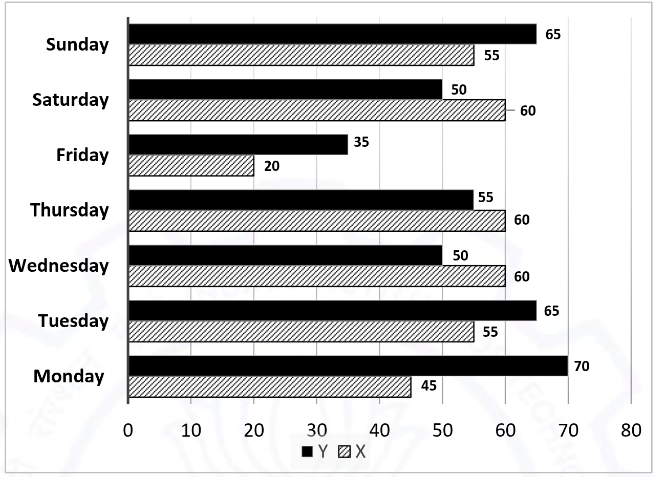
\includegraphics[width=0.5\linewidth]{figs/4.png}
    \caption{}
    \label{fig:2}
\end{figure}

  
Number of days in a week where one student spend at least $10\%$ more than the other:

\begin{enumerate}
\item 4
\item 5
\item 6
\item 7
\end{enumerate}

\hfill (GATE ST 2021) \\

\newpage

\item 
\begin{figure}
    \centering
    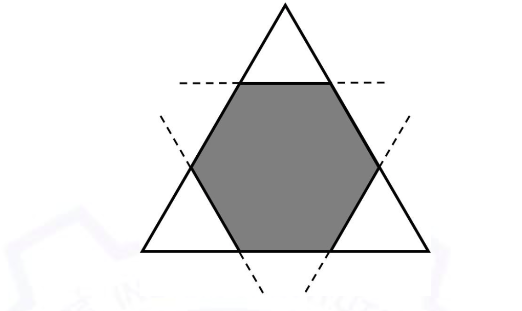
\includegraphics[width=0.5\linewidth]{figs/5.png}
    \caption{}
    \label{fig:3}
\end{figure}

An equilateral triangle is cut at corners to form a regular convex hexagon.  
Ratio of hexagon's area to triangle's area is:

\begin{enumerate}
\item $2:3$
\item $3:4$
\item $4:5$
\item $5:6$
\end{enumerate}

\hfill (GATE ST 2021) \\

\item
Let $X$ be a non-constant positive random variable such that $\mathbb{E}(X) = 9$.  
Which one of the following statements is true?

\begin{enumerate}
\item $\mathbb{E} \brak{\frac{1}{X+1}}  > 0.1$ and $P\brak{X \geq 10} \leq 0.9$
\item $\mathbb{E} \brak{\frac{1}{X+1}}  < 0.1$ and $P\brak{X \geq 10} \leq 0.9$
\item $\mathbb{E} \brak{\frac{1}{X+1}}  > 0.1$ and $P\brak{X \geq 10} > 0.9$
\item $\mathbb{E} \brak{\frac{1}{X+1}}  < 0.1$ and $P\brak{X \geq 10} > 0.9$
\end{enumerate}

\hfill (GATE ST 2021) \\


\item
Let $\{W(t)\}_{t \geq 0}$ be a standard Brownian motion.  
Then the variance of $W\brak{1} W(2)$ equals:
\begin{enumerate}
\item 1
\item 2
\item 3
\item 4
\end{enumerate}

\hfill (GATE ST 2021) \\

\item
Let $X_1, X_2, \dots, X_n$ be a random sample of size $n \ \brak{\geq 2}$ from a distribution with probability density function:
$
f(x; \theta) =
\begin{cases}
\frac{\theta}{x^{\theta+1}}, & x > 1, \; \theta > 0, \\
0, & \text{otherwise}.
\end{cases}
$
Then the method of moments estimator of $\theta$ equals:
\begin{enumerate}
\item $\frac{1}{2\bar{X}}$
\item $\frac{2}{\bar{X}}$
\item $\frac{n}{\sum_{i=1}^n X_i}$
\item $\frac{n}{\sum_{i=1}^n X_i - 2}$
\end{enumerate}

\hfill (GATE ST 2021) \\

\item
Let $\cbrak{ X_1, X_2, \dots, X_n }$ be a sample from $N\brak{\mu,\sigma^2}$, $\ -\infty < \mu < \infty$ and $\sigma > 0$.

P: 95\% confidence interval of $\mu$ when $\sigma$ is known is unique.  
Q: 95\% confidence interval of $\mu$ when $\sigma$ is unknown is \textbf{not} unique.

\begin{enumerate}
\item P only
\item Q only
\item Both P and Q
\item Neither P nor Q
\end{enumerate}
\hfill (GATE ST 2021) \\


\item
Let $X_1, X_2, \dots, X_n$ be a sample from $N\brak{0,\sigma^2}$.  
Test $H_0: \sigma = 1$ against $H_1: \sigma > 1$ at level $\alpha$.

$\mathcal{S}$ has a monotone likelihood ratio in $T_2 = \sum_{i=1}^n X_i^2$ and $H_0$ is rejected if:
\begin{enumerate}
\item $T_1 > \chi_\alpha^2$
\item $T_1 > \chi_{n,1-\alpha}^2$
\item $T_2 > \chi_\alpha^2$
\item $T_2 > \chi_{n,1-\alpha}^2$
\end{enumerate}
\hfill (GATE ST 2021) \\


\item
Let $X$ and $Y$ be binary random variables with $p_{ij} = P\brak{X = i, Y = j}$.  
A sample of size $60$ yields: $n_{11} = 10$, $n_{10} = 20$, $n_{01} = 20$, $n_{00} = 10$.

Under $H_0$: $X$ and $Y$ are independent, the $\chi^2$ test statistic follows:

\begin{enumerate}
\item $\chi^2_{\brak{1}}$ with observed value $\frac{3}{20}$
\item $\chi^2_{\brak{3}}$ with observed value $\frac{20}{3}$
\item $\chi^2_{\brak{1}}$ with observed value $\frac{16}{3}$
\item $\chi^2_{\brak{3}}$ with observed value $\frac{3}{16}$
\end{enumerate}
\hfill (GATE ST 2021) \\


\item
Let $\brak{X,Y}$ follow a bivariate normal distribution with correlation $\rho$ and $\Phi_\rho\brak{0,0}= P\brak{X \leq 0, Y \leq 0}$.  
Kendall's coefficient between $X$ and $Y$ equals:
\begin{enumerate}
\item $4\Phi_\rho\brak{0,0} - 1$
\item $4\Phi_\rho\brak{0,0}$
\item $4\Phi_\rho\brak{0,0} + 1$
\item $\Phi_\rho\brak{0,0}$
\end{enumerate}
\hfill (GATE ST 2021) \\

\item
Consider the simple linear regression model:
$
Y_i = \beta_0 + \beta_1 x_i + \epsilon_i, \quad i = 1, \dots, n, \; n \geq 3
$
with $\bar{x} = \frac{1}{n} \sum_{i=1}^n x_i$, $S_1 = \sum_{i=1}^n (x_i - \bar{x})^2$, $S_2 = \sum_{i=1}^n y_i(x_i - \bar{x})$.  
The variance of $\hat{\beta}_0 + c \hat{\beta}_1$ is:
\begin{enumerate}
\item $\frac{\sigma^2}{n} + \frac{c^2\sigma^2}{S_1}$
\item $\frac{\sigma^2}{n} + \frac{2c^2\sigma^2}{S_1}$
\item $\frac{\sigma^2}{n} + c^2\sigma^2$
\item $\frac{\sigma^2}{c^2 + S_1}$
\end{enumerate}
\hfill (GATE ST 2021) \\

 

\item
Let $X_1,\dots,X_3 \sim N_4\brak{0,\Sigma_1}$ and $Y_1,\dots,Y_4 \sim N_4\brak{0,\Sigma_2}$ independently.  
Define:
$
Z = \Sigma_1^{-\frac12}XX^T\Sigma_1^{-\frac12} + \Sigma_2^{-\frac12}YY^T\Sigma_2^{-\frac12}
$
where $X$ is a $4\times 3$ matrix, $Y$ is a $4\times 4$ matrix.  
Then:
\begin{enumerate}
\item $Z \sim W_4\brak{7, I_4}$
\item $Z \sim W_4\brak{4, I_4}$
\item $Z \sim W_7\brak{4, I_7}$
\item $Z \sim W_7\brak{7, I_7}$
\end{enumerate}
\hfill (GATE ST 2021) \\


 \item
Evaluate:
$
\lim_{n \to \infty} \frac{2n + n 2^n \sin^2\frac{1}{n}}{2n - n 2^n \cos\frac{1}{n}}
$

\hfill (GATE ST 2021) \\
\item
Let
$
I = \int_{0}^{1} \int_{0}^{\sqrt{2 - x^2}} \frac{1}{\sqrt{1 - x^2} \, \sqrt{x^2 + y^2}} \, dy \, dx
$
Find $e^{I + \ln{\sqrt{2}}}$ (round off to 2 decimal places).

\hfill (GATE ST 2021) \\

\item
Let $A = 10I_3$ where $I_3$ is the $3 \times 3$ identity matrix.  
Find the **nullity** of:
$
5A \brak{I_3 + A + A^2}
$

\hfill (GATE ST 2021) \\

\item
Let $A$ be a $2 \times 2$ real matrix with eigenvalues $1$ and $-1$, and corresponding eigenvectors:
$
\myvec{ \sqrt{3} \\ -1 }
\quad \text{and} \quad
\myvec{ 2 \\ 2 }
$
If $A^{2021} = \myvec{ a & b \\ c & d }$,  
find $a+b+c+d$ (round off to 2 decimal places).

\hfill (GATE ST 2021) \\

\item
Let $A$ and $B$ be independent events with $P\brak{B} = \frac{3}{4}$ and $P\brak{A \cup B^c} = \frac12$.  
Find $P\brak{A}$ (round off to 2 decimal places).

\hfill (GATE ST 2021) \\

\item
A fair die is rolled twice independently.  
Let $X$ and $Y$ be the outcomes of the first and second rolls respectively.  
Find $E\brak{X + Y \, | \, \brak{X - Y}^2 = 1}$.

\hfill (GATE ST 2021) \\

\item
Let $X$ have CDF:
$
F\brak{x} =
\begin{cases}
    
0, & x < 1 \\
a - 2c x, & 1 \le x < 2 \\
\frac12, & 2 \le x < 3 \\
1, & x \ge 3
\end{cases}
$
where $a$ and $c$ are constants.  
Given $P\brak{X \leq 1} = \frac15$ and $E\sbrak{X} = 3$,  
find $P\brak{X \in A}$ where $A_n = \sbrak{1+\frac1n,\, 3 - \frac1n}$, $n \ge 1$ and $A = \bigcup_{n=1}^\infty A_n$ (round off to 2 decimal places).

\hfill (GATE ST 2021) \\


\item
If the marginal pdf of the $k$-th order statistic from a sample of size 8 from $U\sbrak{0,2}$ is:
$
f\brak{x} = \frac{7}{32} x \brak{2-x}, \quad 0 < x < 2
$
find $k$.

\hfill (GATE ST 2021) \\

\item
For $a > 0$, let $\brak{ X_n^{\brak{a}} }$ be independent Bernoulli random variables such that:
$
P\brak{X_n^{\brak{a}}} = 1) = \frac{1}{n^\alpha}, \quad P\brak{X_n^{\brak{a} = 0}} = 1 - \frac{1}{n^\alpha}
$
Define $S = \cbrak{ \alpha > 0 : X_n^{\brak{a}} \to 0 \ \text{a.s. as} \ n \to \infty }$.  
Find $\inf S$ (round off to 2 decimal places).

\hfill (GATE ST 2021) \\

\item
Let $\cbrak{X_n}$ be i.i.d. $U\sbrak{0,2}$. For $n \ge 1$, let:
$
Z_n = - \log_e \brak{ \frac{1}{n} \sum_{i=1}^n \brak{2 - X_i} }
$
Find $\lim_{n \to \infty} Z_n$ almost surely (round off to 2 decimal places).
\hfill (GATE ST 2021) \\

\item
A two-state Markov chain $\cbrak{X_n}$ has:
$
P = \myvec{ 0.25 & 0.75 \\ 0.75 & 0.25 }
$
with $P\brak{X_0 = 0} = P\brak{X_0 = 1} = 0.5$. Find:
$
\sum_{k=1}^{100} E\sbrak{\brak{X_{2k}}^{2k}}
$

\hfill (GATE ST 2021) \\

\item
A sample $\sbrak{0,2}$ from Binomial$\brak{n=2,p}$ is used to test $H_0: p = \frac12$ vs $H_1: p \ne \frac12$.  
Find the observed value of the likelihood ratio test statistic (round off to 2 decimal places).

\hfill (GATE ST 2021) \\

\item
Let $X$ have:
$
f\brak{x} = 13x\brak{1-x}\brak{9-x}, \quad 0 < x < 1
$
Find $E\sbrak{ X\brak{X^2 - 15X + 27}}$ (round off to 2 decimal places).

\hfill (GATE ST 2021) \\

\item
Let $\brak{Y, X_1, X_2}$ have mean:
$
\mu = \brak{5,0,2}
$
and covariance:
$
\Sigma =
\myvec{
10 & 0.5 & -0.5 \\
0.5 & 7 & 1.5 \\
-0.5 & 1.5 & 2}
$
Find the multiple correlation coefficient between $Y$ and its best linear predictor using $X_1$ and $X_2$ (round off to 2 decimal places).

\hfill (GATE ST 2021) \\

\item
Let $X_1, X_2, X_3$ be from $N_2\brak{\mu, \Sigma}$ with $\mu$ and $\Sigma$ unknown positive-definite.  
Given sample $\brak{(2,2), (2,2), (5,0)}$, find the $p$-value for testing $H_0: \mu = \brak{0,0}$ vs $H_1: \mu \neq \brak{0,0}$ using the LRT (round off to 2 decimal places)

\item
In the regression model $Y_i = \alpha + \beta x_i + \epsilon_i$,  
with observations: \\
\begin{center}
\begin{tabular}[12pt]{|l|l|}
\hline 
  P.Processes   & 1.Characteristics / Applications \\ \hline
  Q.Gas Metal Arc Welding    & 2.Joining of thick plates \\ \hline
  R.Tungsten Inert Gas Welding &  3.Consumable electrode wire  \\ \hline
  S.Electroslag Welding & 4.Joining of cylindrical dissimilar materials \\ \hline
\end{tabular}
\end{center} 
\bigskip
Find $\alpha + \beta$ (round off to 2 decimal places).

\hfill (GATE ST 2021) \\


\item
Let $f: \mathbb{R} \to \mathbb{R}$ be defined by:
$
f\brak{x} =
\begin{cases}
x^3 \sin x, & x = 0 \ \text{or $x$ irrational}, \\
\frac{1}{p q^3}, & x = \frac{p}{q}, \ p \in \mathbb{Z} \setminus \cbrak{0}, \ q \in \mathbb{N}, \ \gcd\brak{p,q} = 1
\end{cases}
$
Then which one of the following is true?
\begin{enumerate}
\item $f$ is not continuous at $0$
\item $f$ is not differentiable at $0$
\item $f$ is differentiable at $0$ and $f'\brak{0} = 0$
\item $f$ is differentiable at $0$ and $f'\brak{0} = 1$
\end{enumerate}

\hfill (GATE ST 2021) \\

\item
Let $f: \lsbrak{0, \rbrak{\infty}} \to \mathbb{R}$. Which one of the following is true?
\begin{enumerate}
\item If $f$ is bounded and continuous, then $f$ is uniformly continuous.
\item If $f$ is uniformly continuous, then $\lim_{x \to \infty} f\brak{x}$ exists.
\item If $f$ is uniformly continuous, then $g\brak{x} = f\brak{x} \sin x$ is also uniformly continuous.
\item If $f$ is continuous and $\lim_{x \to \infty} f\brak{x}$ is finite, then $f$ is uniformly continuous.
\end{enumerate}

\hfill (GATE ST 2021) \\
\item
Let $f: \mathbb{R} \to \mathbb{R}$ be differentiable with $f\brak{0} = 0$ and $f'\brak{x} + 2f\brak{x} > 0$ for all $x \in \mathbb{R}$. Then which one of the following is true?
\begin{enumerate}
\item $f\brak{x} > 0$ for $x > 0$ and $f\brak{x} < 0$ for $x < 0$
\item $f\brak{x }< 0$ for all $x \neq 0$
\item $f\brak{x} > 0$ for all $x \neq 0$
\item $f\brak{x} < 0$ for $x > 0$ and $f\brak{x} > 0$ for $x < 0$
\end{enumerate}

\hfill (GATE ST 2021) \\
\item
Let $\mathcal{M}$ be the set of $3\times 3$ real symmetric positive definite matrices. Consider  
$
S = \cbrak{ A \in \mathcal{M} : A^{50} - A^{48} = 0 }.
$
The number of elements in $S$ equals:
\begin{enumerate}
\item $0$
\item $1$
\item $8$
\item $8^1$
\end{enumerate}

\hfill (GATE ST 2021) \\

\item
Let $A$ be a $3\times 3$ real matrix such that $I_3 + A$ is invertible and
$
B = \brak{I_3 + A}^{-1}\brak{I_3 - A}.
$
Which one of the following is true?
\begin{enumerate}
\item If $B$ is orthogonal, then $A$ is invertible.
\item If $B$ is orthogonal, then all eigenvalues of $A$ are real.
\item If $B$ is skew-symmetric, then $A$ is orthogonal.
\item If $B$ is skew-symmetric, then $\det(A) = -1$.
\end{enumerate}

\hfill (GATE ST 2021) \\
\item
Let $X \sim \text{Poisson}(\lambda)$ with $E\brak{X^2} = 110$. Which one is NOT true?
\begin{enumerate}
\item $E\sbrak{X} = 10 E\sbrak{\brak{X+1}^{n-1}}$ for all $n \ge 1$
\item $P\brak{X \ \text{even}} = \frac{1 + e^{-20}}{2}$
\item $P\brak{X = k} < P\brak{X = k+1}$ for $k = 0, 1, \dots, 8$
\item $P\brak{X = k} > P\brak{X = k+1}$ for $k = 10, 11, \dots$
\end{enumerate}

\hfill (GATE ST 2021) \\
\item
Let $
X \sim U\brak{-\frac{\pi}{2}, \frac{\pi}{2}}$. Which one is NOT true?
\begin{enumerate}
\item $Y = \cot X$ follows standard Cauchy.
\item $Y = \tan X$ follows standard Cauchy.
\item $Y = -\log_e \brak{\frac{1+ \sin X}{2}}$ has mgf $M(t) = \frac{1}{1-t}$ for $t<1$.
\item $Y = -2\log_e\brak{ \frac{1 + \sin X}{2} }$ follows $\chi^2_{\brak{1}}$.
\end{enumerate}

\hfill (GATE ST 2021) \\
\item
Let $\Omega = \brak{1,2,3,\dots}$ with $P(\{n\}) = a_n$. Which one is NOT true?
\begin{enumerate}
\item $\lim_{n\to\infty} a_n = 0$
\item $\sum_{n=1}^\infty \sqrt{a_n}$ converges
\item For any $k$, there exist disjoint $A_1, \dots, A_k$ with $P\brak{\cup_{i=1}^k A_i} < 0.001$.
\item There exists an increasing sequence $\cbrak{A_i}$ with $P\brak{\cup_{i=1}^\infty A_i} < 0.001$.
\end{enumerate}

\hfill (GATE ST 2021) \\
\item
Let $\brak{X,Y}$ have pdf $f_{X,Y}(x,y) = \frac{4}{3}\brak{x+y}^3$ for $0 < x < 1$, $0 < y < 1$, $0$ otherwise. Which is NOT true?
\begin{enumerate}
\item The probability density function of $X+Y$ is $f_{X+Y}\brak{z} = \frac{4}{3} z^3 \brak{z-2}$ for $0<z<2$
\item $P\brak{X+Y > 4} = \frac{3}{4}$
\item $E\brak{X+Y} = 4 \log_e 2$
\item $E\brak{Y \mid X=2} = 4$
\end{enumerate}

\hfill (GATE ST 2021) \\
\item
Let $X_1, X_2, X_3$ be uncorrelated with var = $\sigma^2$. Let:
$
Y_1 = 2X_1 + X_2 + X_3,\quad Y_2 = X_1 + 2X_2 + X_3,\quad Y_3 = X_1 + X_2 + 2X_3.
$
P: Sum of eigenvalues of Cov $\brak{Y_1,Y_2,Y_3}$ is $18\sigma^2$.  
Q: Corr$\brak{Y_1,Y_2}$ = Corr $\brak{Y_2,Y_3}$.
\begin{enumerate}
\item P only
\item Q only
\item Both P and Q
\item Neither P nor Q
\end{enumerate}

\hfill (GATE ST 2021) \\


\item
Let $\cbrak{X_n}$ be a Markov chain. Which one is true?
\begin{enumerate}
\item There is at least one recurrent state.
\item If there is an absorbing state, there exists at least one stationary distribution.
\item If all states are positive recurrent, there is a unique stationary distribution.
\item If irreducible, $S = \sbrak{1,2}$, and $\sbrak{\pi_1,\pi_2}$ stationary, then $\lim_{n\to\infty} P\brak{X_n=i \mid X_0=i} = \pi_i$.
\end{enumerate}

\hfill (GATE ST 2021) \\

\item
Customers arrive via Poisson($10$), male/female equally likely. $N\brak{t}$ = total arrivals by $t$. Which one is NOT true?
\begin{enumerate}
\item $P\brak{S_2 \le 1} = 25 \int_0^1 s e^{-5s} ds$, where $S_2$ = time of 2nd female.
\item $P\brak{M\brak{2} = 0 \mid M\brak{1} = 1} = \frac13$.
\item $E\sbrak{N\brak{t}^2}= 100t^2 + 10t$.
\item $E\sbrak{N\brak{t}N\brak{2t}} = 200t^2 + 10t$.
\end{enumerate}
\hfill (GATE ST 2021) \\

\item
Let $X_{\brak{1}} < \dots < X_{\brak{5}}$ from $U\sbrak{0,\theta}$. True?
\begin{enumerate}
\item P only
\item Q only
\item Both P and Q
\item Neither P nor Q
\end{enumerate}
\hfill (GATE ST 2021) \\

\item
Let $X_i \sim f\brak{x;\theta} = \frac{1}{\theta} e^{-x/\theta}$, $x>0$. Then $E\brak{X_{\brak{1}} \mid T}$ equals:
\begin{enumerate}
\item $\frac{T}{n^2}$

\item $\frac{T}{n}$
\item $\frac{\brak{n+1}T}{2n}$
\item $\frac{\brak{n+1}^2T}{4n^2}$
\end{enumerate}
\hfill (GATE ST 2021) \\

\item
Let $X_i \sim U\sbrak{-\theta,\theta}$. True?
\begin{enumerate}
\item P only
\item Q only
\item Both P and Q
\item Neither P nor Q
\end{enumerate}
\hfill (GATE ST 2021) \\
\item
EDF $S_n\brak{x}$ from bounded support $\brak{a,b}$. Which one is NOT true?
\begin{enumerate}
\item $\limsup_{n\to\infty} \sup_x |S_n\brak{x}-F\brak{x}| = 0$ a.s.
\item For fixed $x$, $\sqrt{n}\frac{S_n(x)-F(x)}{\sqrt{S_n(x)(1-S_n(x))}} \to_d N(0,1)$
\item $\text{Cov}\brak{S_n(x), S_n(y)} = \frac{F\brak{x}\brak{1-F\brak{y}}}{n}$
\item If $Y_n = \sup_x \brak{S_n(x)-F(x)}^2$, then $4n Y_n \to_d \chi^2_{\brak{2}}$.
\end{enumerate}
\hfill (GATE ST 2021) \\


\item
Let $\brak{X_1,\dots,X_4} \sim N_4\brak{\mu,\Sigma}$ with  
$\mu = \brak{1,0,0,0}$, $\Sigma = \myvec{ 1 & 0.2 & 0 & 0 \\ 0.2 & 2 & 0 & 0 \\ 0 & 0 & 1 & 0.2 \\ 0 & 0 & 0.2 & 1 }$.  
Which one is true?
\begin{enumerate}
\item $\sbrak{\brak{X_1+X_2}^2 + \brak{X_3+X_4-1)^2}} \sim \chi^2_{(2)}$
\item $\sbrak{\brak{X_1+X_3-1}^2 + \brak{X_2+X_4-1}^2}\sim \chi^2_{(2)}$
\item $E\sbrak{\frac{X_1+X_2-1}{X_3+X_4-1}}$ is not finite
\item $E\sbrak{ \frac{X_1+X_2+X_3+X_4-2}{X_1+X_2-X_3-X_4} }$ is not finite
\end{enumerate}
\hfill (GATE ST 2021) \\

\item
Let $Y \sim N_8\brak{0,I_8}$ and $Y^T\Sigma_1Y \sim \chi^2_{\brak{3}}$, $Y^T\Sigma_2Y \sim \chi^2_{(4)}$, independent. True?
\begin{enumerate}
\item P only
\item Q only
\item Both P and Q
\item Neither P nor Q
\end{enumerate}
\hfill (GATE ST 2021) \\


\item
Let $(X,Y)$ have joint pdf:
$
f_{X,Y}\brak{x,y} = \frac{1}{\pi} e^{-\brak{2x - 3x^2 - 2y^2}}, \quad -\infty < x,y < \infty.
$
Find $8 \, E\brak{XY}$.
\hfill (GATE ST 2021) \\

\item
Let $f: \mathbb{R} \times \mathbb{R} \to \mathbb{R}$ be:
$
f\brak{x,y}= 8x^2 - 2y.
$
If $M$ and $m$ are the maximum and minimum values of $f$ on $\cbrak{ \brak{x,y} : x^2 + y^2 = 1 }$,  
find $M - m$ (round off to 2 decimal places).
\hfill (GATE ST 2021) \\


\item
Let 
$
A = \sbrak{a, u_1, u_2, u_3}, \quad
B = \brak{b, u_1, u_2, u_3}, \quad
C = \brak{u_2, u_3, u_1, a+b}
$
be $4\times 4$ real matrices where $a,b,u_1,u_2,u_3$ are $4 \times 1$ real column vectors.  
If $\det(A) = 6$ and $\det(B) = 2$, find $\det\brak{A+B} - \det\brak{C}$.
\hfill (GATE ST 2021) \\
\item
A random variable $X$ has mgf:
$
M\brak{t} = \frac{e^t - 1}{t\brak{1-t}}, \quad t < 1.
$
Find $P\brak{X > 1}$ (round off to 2 decimal places).
\hfill (GATE ST 2021) \\
\item
Let $\brak{ X_n }$ be i.i.d. $\text{Uniform}(0,3)$.  
Let $Y$ be an independent random variable with:
$
P\brak{Y = k} = \frac{1}{e-1} \cdot \frac{1}{k!}, \quad k = 1,2,\dots
$
Find $P\brak{ \max\brak{ X_1,\dots,X_Y } \le 1 }$ (round off to 2 decimal places).

\hfill (GATE ST 2021) \\


\item
Let  $X_n$ be i.i.d. with pdf:
$
f(x) = e^{-x}, \quad x > 0,
$
and $0$ otherwise.  
Let $X_{(n)} = \max\cbrak{ X_1,\dots,X_n }$. If 
$
Z = X_{(n)} - \log n
$
converges in distribution as $n \to \infty$, find the **median** of $Z$ (round off to 2 decimal places).

\hfill (GATE ST 2021) \\

\item
Customers arrive at a park via Poisson process with rate $1/\text{unit time}$.  
Service times are i.i.d. exponential with rate $1$. At a certain time, there are 10 visitors in the park.  
If $p$ is the probability that exactly two more arrivals occur before the next departure, find $1/p$.

\hfill (GATE ST 2021) \\

\item
Given the sample $\{0.90, 0.50, 0.01, 0.95 \}$ from:
$
f(x) = \frac{\theta\, x^{\theta - 1}}{1 - \brak{2^{\theta} - 1}/\brak{1- \theta}}, \quad 0 < x < 1, \ 0.5 \le \theta < 1,
$
find the MLE of $\theta$ (round off to 2 decimal places).

\hfill (GATE ST 2021) \\
\item
A sample of size $100$ from $N\brak{\mu,9}$ yields $\bar{X} = 5.608$.  
Given $\Phi\brak{1.96}= 0.975$, $\Phi\brak{1.64} = 0.95$,  
find the $p$-value for testing $H_0: \mu = 5.02$ vs $H_1: \mu \neq 5.02$ using the UMPU test  
(round off to 3 decimal places).
\hfill (GATE ST 2021) \\
\item
Let $X$ be a discrete random variable with probability mass function

\begin{tabular}[12pt]{ |c| c| } 
    \hline
    {Group I: Aircraft mode} & {Group II: Property}\\ 
    \hline
    P: Short period mode & 1: Coupled roll-yaw oscillations\\
    \hline 
    Q: Wing rock & 2: Angle of attack remains constant \\
    \hline
    R: Phugoid mode & 3: Roll oscillations \\
    \hline   
    S: Dutch roll & 4: Speed remains constant\\
    \hline
\end{tabular}
  \bigskip

To test $H_0: p = p_0$ against $H_1: p = p_1$, the power of the most powerful test of size 0.05 based on $X$ equals (round off to 2 decimal places).
\hfill (GATE ST 2021) \\
\item
Let $X_1,\dots,X_{10}$ be from $f_\theta\brak{x} = f\brak{x-\theta}$ where $f$ is symmetric about $0$.  
For testing $H_0: \theta = 1.2$ vs $H_1: \theta \neq 1.2$,  
let $T_+$ be the Wilcoxon signed-rank statistic and $\eta = P\brak{T_+ < 50 \mid H_0}$.  
Find $32 \eta$ (round off to 2 decimal places).
\hfill (GATE ST 2021) \\
\item
In the regression:
$
Y_i = \beta_0 + \beta_1 x_{1,i} + \dots + \beta_{22} x_{22,i} + \epsilon_i, \quad i=1,\dots,123,
$
given SSR = 338.92, SST = 522.30,  
find $100\, R_{\text{adj}}^2$ (round off to 2 decimal places).
\hfill (GATE ST 2021) \\
\end{enumerate}
\end{document}
